\documentclass[addpoints]{exam}
\usepackage{amsmath,amsthm,amssymb,url}

\usepackage{algorithm}
\usepackage{algorithmic}
\usepackage{graphicx}
\usepackage{float}
\usepackage[pdftex]{hyperref}


\newtheorem{lemma}{Lemma}[section]
\newcommand{\var}{\text{Var}}
\title{CS 6150: HW4}
\date{Due Date: }
\begin{document}
\maketitle
\begin{center}
\fbox{\fbox{\parbox{5.5in}{\centering
This assignment has \numquestions\ questions, for a total of \numpoints\
points.
Unless otherwise specified, complete and reasoned arguments will be
expected for all answers. 
}}}
\end{center}

\qformat{Question \thequestion: \thequestiontitle\dotfill \textbf{[\totalpoints]}}
\pointname{}
\bonuspointname{}
\pointformat{[\bfseries\thepoints]}

\printanswers

\begin{center}
  \gradetable
\end{center}
\newpage



\begin{questions}


\titledquestion{Cycle Cover}[20]
A cycle cover $C$ of a directed graph $G(V,E)$ is a collection of
vertex-disjoint directed cycles so that each vertex in V belongs to
some cycle in $C$.

Give a polynomial time algorithm to compute a cycle cover of a given
directed graph, or correctly report that one does not exist.
\begin{solution}
A cycle cover $C$ of a directed graph $G(V,E)$ is a collection of
vertex-disjoint directed cycles so that each vertex in V belongs to
some cycle in $C$. In order to find cycle cover in graph $G(V,E)$ we will perform the following steps:

\begin{parts}
\part Transform every vertex $v \in V$ of graph $G=(V,E)$, into two parts $u_i$ and $v_i$. 
\part Using $u_i$ and $v_i$ form a bipartite graph $H$.
\part Connect the vertex $u_i$ and $v_j$ of the graph $H$ as represented in the directed graph $G$.
\part Find perfect matching in $H$. (Every vertex of the graph is only connected by a single edge in the matching.)
\part This proves that every perfect match in graph $H$ corresponds to a cycle cover in the graph $G$.
\part If perfect match not found then no cycle cover exists.
\end{parts}

The algorithm will take $O(n)$ to convert graph $G$ to a bipartite graph $H$. In order to find a perfect matching we will require $O(n)$ time. Hence my algorithm can be compute a cycle cover of a directed graph in polynomial time or correctly report that one does not exist.

\emph{http://www.cs.cmu.edu/~avrim/451f13/recitation/rec1016.txt}\\
\emph{Collaboration with Shweta, Sunny and Yogesh}
\end{solution}

\titledquestion{Attend all lectures}[20]
There are $n$ lectures with start time $s_{i}$, end time $e_{i}$
and $t_{ij}$ being the time spent in going from lecture $i$ to $j$.
Now a group of students wants to attend all of the lectures by
sending no more than one student to each lecture. Assume $s_{i}, e_{i},
t_{ij}$ are all positive integers.

Find an algorithm that minimizes number of students covering all the
lectures.
\begin{solution}
Let $C_i$ denote a lecture $i$ with start $\&$ end time as $s_{i}$ and $e_{i}$ respectively. We can visualise the original problem as a flow problem as follows. 

We will assume each lecture $C_i$ as a node. Each lecture $C_i$ can be visualized as pair of nodes marked as $C_{i[in]}$ and $C_{i[out]}$ where they are connected by an edge whose value is defined by $1$. Let $S$ and $T$ be source and sink. We will send students from source. $C_i$ will be connected to $C_j$ only when the condition $s_j \geq e_i + t_{ij}$ is satisfied. The value of the edge is defined as $1$. All others are connected to source and sink directly. Hence taking all of the assumptions above we have reduced the original problem to a flow problem. Every student from source will take the longest path to sink, hence covering the maximum number of lectures.

Now apply the Ford-Fulkerson algorithm to the graph while maximizing coverage of nodes for each student. Hence the residual graph after each flow will have a shorter path left. Thus the number of paths that we get is the minimum number of students required to cover all lectures.\\

\emph{Collaboration with Shweta, Sunny and Yogesh}
\end{solution}


\titledquestion{Monotone path}[20]

Solve all parts of question 2 in
\url{http://web.engr.illinois.edu/~jeffe/teaching/algorithms/notes/25-maxflowext.pdf}

Breakdown is $5$ + $5$ + $10$.

\begin{figure}[H]
  \centering
  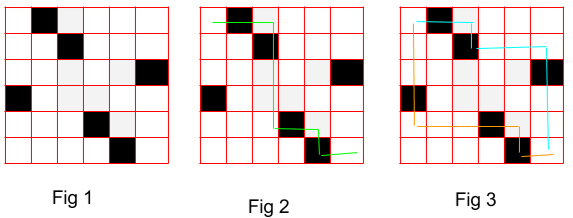
\includegraphics[width=0.75\textwidth]{algo}\\
\end{figure}
\begin{solution}
\begin{enumerate}
\item
Algorithm to find a monotone path that covers the largest number of marked cells:\\
We will apply a programming approach where we will start from cell $(1,1)$ to $(n,n)$. Each cell is denoted by $P = (i,j)$:\\

Start at $i = 1, j = 1$;\\
While$(i \neq n$ $\&$ $j\neq n)$:\\
$\rightarrow$ Scan the current row towards the right to find the number of marked cells denoted by $R$\\
$\rightarrow$ Scan the column towards down to find the number of marked cells denoted by $D$\\
$\rightarrow$if $R > D$\\
$\rightarrow$	\ \ \ \ \ $j \gets j+1$\\
$\rightarrow$   else\\
$\rightarrow$	\ \ \ \ \ $i \gets i+1$\\
    
\item
Greedy approach will fail in current $6X6$ example.

Figure 1 is the input grid. Middle image (Figure $2$) shows the greedy path; in fact any greedy monotone path covers the same four marked cells. If we start with a greedy path, we need two more monotone paths to cover the other two marked cells. Figure $3$ on the right shows that all marked cells can be cover using just two monotone paths.

\item
We will try to find the solution to this problem by reducing the problem to the flow with demand problem.
We will create a directed flow network $G$ with both capacity and edges:
\begin{enumerate}
\item
Graph $G$ will contain two vertices $u_{i,j}$ and $v_{i,j}$ for an array index $M_{[i,j]}$.It also has source vertex $s$ and the target vector is $v{n,n}$.
\item
$u_{i,j}$ has a directed edge to $v_{i,j}$ with a capacity zero. it has demand $1$ if $M_{[i,j]} = true$
else it has demand $0$
\item
$v_{i,j}$ has an directed edge to each of his neighbor $u_{i+1,j}$ and $u_{i,j+1}$ with demand and capacity as zero.
\item
$s$ is connected to $u_{1,1}$ with capacity $k$.
\end{enumerate}
We construct a directed flow network $G$ with both capacities and demands on the edges, as follows:\\
\begin{enumerate}
\item
$G$ has two vertices $u_{i,j}$ and $v_{i,j}$ for each pair of indices $i$ and $j$, plus an additional source vertex $s$. The target vertex is $v_{n,n}$.
\item
Each vertex $u_{i,j}$ has an outgoing edge to its partner vertex $v_{i,j}$. Each partner edge has \emph{demand} $1$ if $M[i,j] = \emph{True}$ and demand $0$ otherwise; partner edges do not have capacities.
\item
Each vertex $v_{i,j}$ has outgoing edge to its right neighbour $u_{i,j+1}$, and its downward neighbor $u_{i+1,j}$ if they exist.Neighbor edges have neither demands nor capacities.
\item Finally there is an edge $s \rightarrow u_{1,1}$ with capacity k. 
\end{enumerate}

Each monotone path through the grid is represented by a directed path in $G$. Conversely, every directed path in $G$ represents a monotone path through the grid.If we can cover all the marked cells by $k$ paths in the Grid there is a flow in the graph network from $s$ to $v_{n,n}$. Similarly if there is a flow $({s,t})$ in the graph network with the value $k$ we can say that that flow can gives us $k$ monotone paths from $M_{[1,1]}$ to $M_{n,n}$ by covering all the marked cells.
Hence we can solve the problem by finding the maximum flow in the graph $G$.\\

The network $G$ has $O(n^2)$ vertices and edges, and we can easily construct it in $O(n^2)$ time. Computing a maximum flow in a network with both capacities and demands requires $O(V.E\log V) = O(n^4 \log n)$ time using the most efficient max-flow algorithms. Thus, the overall running time of this algorithm is $O(n^4 \log^2 n)$.

\emph{https://github.com/iveney/cs573/blob/master/hw5/hw5sol-official.pdf}\\
\emph{Collaboration with Shweta, Sunny and Yogesh}
\end{enumerate}
\end{solution}

\titledquestion{Vertex-disjoint paths}[20]
Given a square grid ($n$ x $n$) like the following figure, and a set of $m
\leq n^{2}$ distinct points marked in black, devise an algorithm to
determine whether there exists $m$ vertex-disjoint paths starting at
those marked points and ending at points at the boundary of the grid.

\begin{figure}[H]
  \centering
  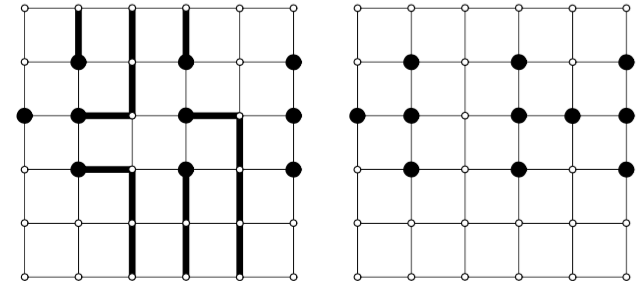
\includegraphics[width=0.75\textwidth]{grid}\\
  \caption{In the left grid there exists such a path, but in the right
  grid there isn't}
\end{figure}

\begin{solution}

We reduce the problem to the “maximum flow problem in a network with edge and vertex capacities”. The reduction consists in transforming the input grid of the problem into a flow network $G = (V, E)$. Initially there are $m$ points marked as black on the grid and $4n-4$ boundary points. The construction of $G = (V, E)$ will be as follows:
\begin{enumerate}
\item Take a source vertex $s$ and connect $s$ to each of the $m$ black points.
\item Take another vertex $t$ as sink and connect each of the $4n-4$ boundary points to t.
\item Each adjacent cell in the grid can be considered as adjacent nodes $u$ and $v$ in Graph $G$ connected with two directed edges $(u, v)$ and $(v, u)$ in G.
\item Assign edge capacity as $1$ to each edge in $G$ and every vertex capacity as $1$ to each vertex in G.
\end{enumerate}

To determine whether there exists $m$ vertex-disjoint paths, we will start at each of the black marked points and end at the boundary points.The flow sent from source $s$ should be equal to the flow received at sink $t$ and maximum flow should be $m$.
i.e, the maximum flow in $G$ should be $m$, then there exists $m$ vertex-disjoint paths.

For this algorithm to give the vertex-disjoint paths, assign every edge capacity as $1$ from marked point to boundary points.Using Ford-Fulkerson algorithm we will find flow sequentially from the source. Every time a path is used we will remove it. If by the end of it we get maximum flow equal to $m$, thus we have got $m$ vertex disjoint paths.\\

The running time cost of Ford-Fulkerson method on $G$, the running time is $O((V+E)|f^*|)$. The input grid has $n^2$ points and $2n^2-2n$ undirected edges. Hence, $G$ has $2 + n^2 = O(n^2)$ vertices and $m+ (4n-4) + 2(2n^2 -2n) = m+ 4n^2 -4 = O(n^2)$ (directed) edges. Hence, the running time is $O((V+E)|f^*|)$. In the given problem, $|f^*| \le (4n - 4)$ and $|E| + |V | = O(n^2)$. Hence, a tighter bound for the running time is $O((E + V ) · |f^*|) = O(n^3)$.\\

\emph{Solution found at : http://webcourse.cs.technion.ac.il/234247/Spring2006/ho/WCFiles/\\The\%20Escape\%20Problem.pdf}\\
\emph{Collaboration with Shweta, Sunny and Yogesh}
\end{solution}

\titledquestion{Uniqueness of mincut}[20]
Given an $s$-$t$ flow network, find a polynomial time algorithm to
determine whether the  mincut is unique.
\begin{solution}
Using the Ford-Fulkerson's Algorithm, lets compute a minimum s-t cut $S$, and its capacity is denoted by $|S|$. Let $e_1, e_2, . . . , e_m$ be the edges in minimum cut $S$. After finding minimum cut $S$, we will try to verify that whether it is unique or not. Lets find another minimum cut in $G$ denoted by $S_i$. If $|S|$ and $|S_i|$ are same in all aspects then the $S$ is unique, else not. To reverify we can look at it in this way. Min cut is the bottleneck cut which is the max flow of a network, i.e. that amount of flow received at sink is that highest. Now if we increase the capacity of each edge in $S$ one by one and the max flow does not increase, then it mean that there is another possible edge which could contribute to a min cut, thus maximizing flow. 

Alternatively we could look at it as, once calculating a min cut from source, we will calculate a min cut from sink. If both the min cuts are identical than the min-cut is unique.

As there are possible $m$ edges in the mincut, hence linearly increasing the capacity of a edge in $S$ to verify increase of flow will take us atmost $m + 1$ computing of minimum cuts, and therefore the algorithm runs in polynomial time.\\

\emph{http://web.stanford.edu/class/cme305/Midterm/pmidtermIsoln.pdf}\\
\emph{Collaboration with Shweta, Sunny and Yogesh}
\end{solution}

\end{questions}

\end{document}

%%% Local Variables:
%%% mode: latex
%%% TeX-master: t
%%% End:
